\documentclass[11pt,a4paper]{article}
\usepackage{lmodern}
\usepackage{float}
\usepackage{amssymb,amsmath}
\usepackage{multicol}
\usepackage{pgfgantt}
\usepackage{fontawesome}
\usepackage{ifxetex,ifluatex}
\usepackage{graphicx}
\usepackage{eso-pic}
\usepackage{wallpaper}
\usepackage{fixltx2e} % provides \textsubscript
\usepackage{lipsum, babel}
\ifnum 0\ifxetex 1\fi\ifluatex 1\fi=0 % if pdftex
  \usepackage[T1]{fontenc}
  \usepackage[utf8]{inputenc}
\else % if luatex or xelatex
  \ifxetex
    \usepackage{mathspec}
  \else
    \usepackage{fontspec}
  \fi
  \defaultfontfeatures{Mapping=tex-text,Scale=MatchLowercase}
  \newcommand{\euro}{€}
\fi
% use upquote if available, for straight quotes in verbatim environments
\IfFileExists{upquote.sty}{\usepackage{upquote}}{}
% use microtype if available
\IfFileExists{microtype.sty}{%
\usepackage{microtype}
\UseMicrotypeSet[protrusion]{basicmath} % disable protrusion for tt fonts
}{}
\usepackage[margin=0.787402in]{geometry}
\makeatletter
\@ifpackageloaded{hyperref}{}{%
\ifxetex
  \usepackage[setpagesize=false, % page size defined by xetex
              unicode=false, % unicode breaks when used with xetex
              xetex]{hyperref}
\else
  \usepackage[unicode=true]{hyperref}
\fi
}
\@ifpackageloaded{color}{
    \PassOptionsToPackage{usenames,dvipsnames}{color}
}{%
    \usepackage[usenames,dvipsnames]{color}
}
\makeatother
\hypersetup{breaklinks=true,
            bookmarks=true,
            pdfauthor={},
            pdftitle={},
            colorlinks=true,
            citecolor=blue,
            urlcolor=blue,
            linkcolor=magenta,
            pdfborder={0 0 0}
            }
\urlstyle{same}  % don't use monospace font for urls
\usepackage{graphicx,grffile}
\makeatletter
\def\maxwidth{\ifdim\Gin@nat@width>\linewidth\linewidth\else\Gin@nat@width\fi}
\def\maxheight{\ifdim\Gin@nat@height>\textheight\textheight\else\Gin@nat@height\fi}
\makeatother
% Scale images if necessary, so that they will not overflow the page
% margins by default, and it is still possible to overwrite the defaults
% using explicit options in \includegraphics[width, height, ...]{}
\setkeys{Gin}{width=\maxwidth,height=\maxheight,keepaspectratio}
\setlength{\parindent}{0pt}
\setlength{\parskip}{6pt plus 2pt minus 1pt}
\setlength{\emergencystretch}{3em}  % prevent overfull lines
\providecommand{\tightlist}{%
  \setlength{\itemsep}{0pt}\setlength{\parskip}{0pt}}
\setcounter{secnumdepth}{0}

\date{}

% Redefines (sub)paragraphs to behave more like sections
\ifx\paragraph\undefined\else
\let\oldparagraph\paragraph
\renewcommand{\paragraph}[1]{\oldparagraph{#1}\mbox{}}
\fi
\ifx\subparagraph\undefined\else
\let\oldsubparagraph\subparagraph
\renewcommand{\subparagraph}[1]{\oldsubparagraph{#1}\mbox{}}
\fi
\usepackage[para]{footmisc}

\newcommand*{\plogo}{\fbox{$\mathcal{PL}$}} % Generic publisher logo
\ThisCenterWallPaper{1}{images/Marrus_orthocanna.jpg}
%----------------------------------------------------------------------------------------
%    TITLE PAGE
%----------------------------------------------------------------------------------------

\newcommand*{\titleGP}{\begingroup % Create the command for including the title page in the document
{\color{white}\begin{itemize}
\centering % Center all text
\vspace*{\baselineskip} % White space at the top of the page

\rule{\textwidth}{1.6pt}\vspace*{-\baselineskip}\vspace*{2pt} % Thick horizontal line
\rule{\textwidth}{0.4pt}\\[\baselineskip] % Thin horizontal line

{\LARGE Nano-medicine logic design \\ using \\[0.3\baselineskip] ~a bio-inspred robotic platform and morphological computation}\\[0.2\baselineskip] % Title

\rule{\textwidth}{0.4pt}\vspace*{-\baselineskip}\vspace{3.2pt} % Thin horizontal line
\rule{\textwidth}{1.6pt}\\[\baselineskip] % Thick horizontal line

\scshape % Small caps
Robotics Research Preparation \\ % Tagline(s) or further description
Assignment: Research Plan \\[\baselineskip] % Tagline(s) or further description
Thursday, 31\textsuperscript{st} March 2017\par % Location and year

\vspace*{2\baselineskip} % Whitespace between location/year and editors

Edited by \\[\baselineskip]
{\Large Asheesh Sharma\par} % Editor list
\textbf{Candidate: 33074, Student: 1562159}\\
{\itshape University of Bristol \\ United Kingdom\par} % Editor affiliation
{\Large \faGithub}
\vfill % Whitespace between editor names and publisher logo

\begin{figure}[htbp]
\centering
\resizebox{0.2\textwidth}{!}{
\includegraphics{images/whitelogo.png}}
\end{figure} \\[0.3\baselineskip] % Publisher logo
{\scshape 2017} \\[0.3\baselineskip] % Year published
\par % Publisher
\end{itemize}}
\endgroup}




\begin{document}
\pagestyle{empty} % Removes page numbers
\titleGP % This command includes the title page

\newpage

\hypersetup{linkcolor=black}
\setcounter{tocdepth}{3}
\tableofcontents
\clearpage

\pagestyle{plain}

\section{Aims and Objectives}\label{aim}
\subsection{Aim}
\begin{enumerate}
     \item To develop a robotic platform for simulating nanoparticle swarms in a targeted drug delivery scenario.
     \item To develop a generalised nanoparticle swarm model.
   \end{enumerate}
\subsection{Objectives}
\begin{enumerate}
   \item Design and build
   \begin{enumerate}
     \item a mechanical medium for local communication in the robotic swarm.
     \item a sensory system
     \item a central pattern generator (CPG) to couple sensory information with the mechanical medium.  
     \item a specialised (i.e. with different abilities) swarm of aquatic robots. 
   \end{enumerate}
   \item Study
   \begin{enumerate}
     \item the feasibility of morphological computation in nanoparticle swarms using the platform.
     \item the emergent behaviour with different types of obstacle courses representing different tissues.
     \item the effects of hierarchical structure and specialisation on self-organisation in the robotic swarm.  
   \end{enumerate}
 \end{enumerate}


\newpage
\begin{center}
\section{Motivation}\label{motivation}
\end{center}
\begin{multicols}{2}
\subsection{A generalised nanoparticle swarm architecture for targeted drug delivery}\label{gen}
Targeted drug delivery is one of the major challenges in medicine and bio-engineering. It is a method of medication for promoting the concentration of therapeutic drugs to specific organs without affecting the functioning of other body systems\cite{muller2004challenges}. For example, bacteria like \emph{Magnetococcus marinus} have been shown to efficiently deliver drugs to specific targets. This bacteria tends to swim towards lower oxygen concentration when triggered with a magnetic field. Using a programmed magnetic field, researchers were able to direct the bacteria towards tumours, while maintaining distance from healthy cells (oxygen rich) \cite{felfoul2016magneto}. Similarly, many other methods have been proposed for delivering medicines to a target tissue but none of them has attracted more attention than the field of nano-medicine\cite{farokhzad2009impact}. This approach of is based on the novel idea of designing nanoparticles (size, shape, charge, material, coating, activation etc.). Although there is a diverese range of desgn variable, many hurdles arise in the logical design of nanomedicine. Firstly, it becomes harder to predict the emergent behaviour of nanoparticles as the population increases. Secondly, as the population
is increased, the designed behaviour may not scale accordingly \cite{chowdhury2015controlling}\cite{kim2015imparting}. Thirdly, the design of nanoparticle may not generalise for different types of tissue, drug and deployment channel\cite{li2011mathematical}. 

To overcome these hurdles, researchers have devised many
targeting strategies. If the circulation time is directly related to the drug's success (passive targeting), the nanoparticles can be made to prolong the interaction of drug \cite{van2007poly}. To make the same nanoparticle specific to the target, it can be equipped with ligands which are only complimentary to the receptors (active targeting) of the
target tissue \cite{galvin2012nanoparticle}. However, both of these strategies are not sufficient enough to predict the emergent behaviour of nanoparticles interacting in complex tumour environments. In order to build a prediction model, a systems approach can be employed by assuming that the nano-particles are interacting locally. This, in effect, can lead to emergent behaviour which is commonly seen in self-organised systems like swarms \cite{hauertnisms}. With the immediate realisation of the link between bio-mimetic nano-particles and swarms, it can also be assumed that the nanoparticles have to be hierarchical\footnote{It should also be noted that the hierarchical order can change.} and specialised. For instance, a group of nanoparticles (bulldozers\footnote{Bulldozer particles are equipped with ligands which are complementary to the specific receptors of a tissue.}) have to penetrate a tumour before another group of particles (satellites\footnote{Satellite particles are loaded with drugs. Each of these particles has a core which is surrounded by drug molecules.}) can deliver the drug. Since the interactions are dependent on the type of tissue and the design variables are physical, the local communication must be mechanical in form. Furthermore, these mechanical ``links'' also serve the purpose of the computation required for the entire population to localise\footnote{Particles can change their state at the target tissue} when they reach the target.

Therefore it can be seen that the above realisation naturally converges towards the basic principles of a bio-inspired design \cite{pfeifer2007self}. Firstly, it becomes clear that the behaviour is not solely dependent on its internal controlled. More specifically, the outcome of internal control is not the only entity which controls the behaviour of this system. In other words, the system (not in ideal conditions) is also affected by its morphology which includes senses, the shape of the body and its materialistic properties. For instance, when designing a passive nanoparticle, it is assumed that the nanoparticle are solely dependent on its internal control, however, they are known to be less effective because of the assumption fails to capture the role of morphology. Secondly, physical constraints on the morphology of a system define the dynamics of interaction with the environment. For example, dynamics of nanoparticles in the blood stream is different than in tumour. Thus, there is a direct link between embodiment and information. Therefore, sensory information and body morphology share the regularities of control to cope with the environment. Finally, together, physical constraints, morphology, and sensory inputs give rise to self-organization resulting in an emergent behaviour. 

Based on these design principles, a simple nanoparticle system is proposed which tries to tackle the issues of scalability and control by exploiting the morphology of the system (Figure 1). Although the actual implementation of the system is out of the scope of the project, a robotic platform will be designed in order to demonstrate the capability of this system and its dynamic properties.

\end{multicols}


\newpage
\begin{figure}[htbp]
\centering
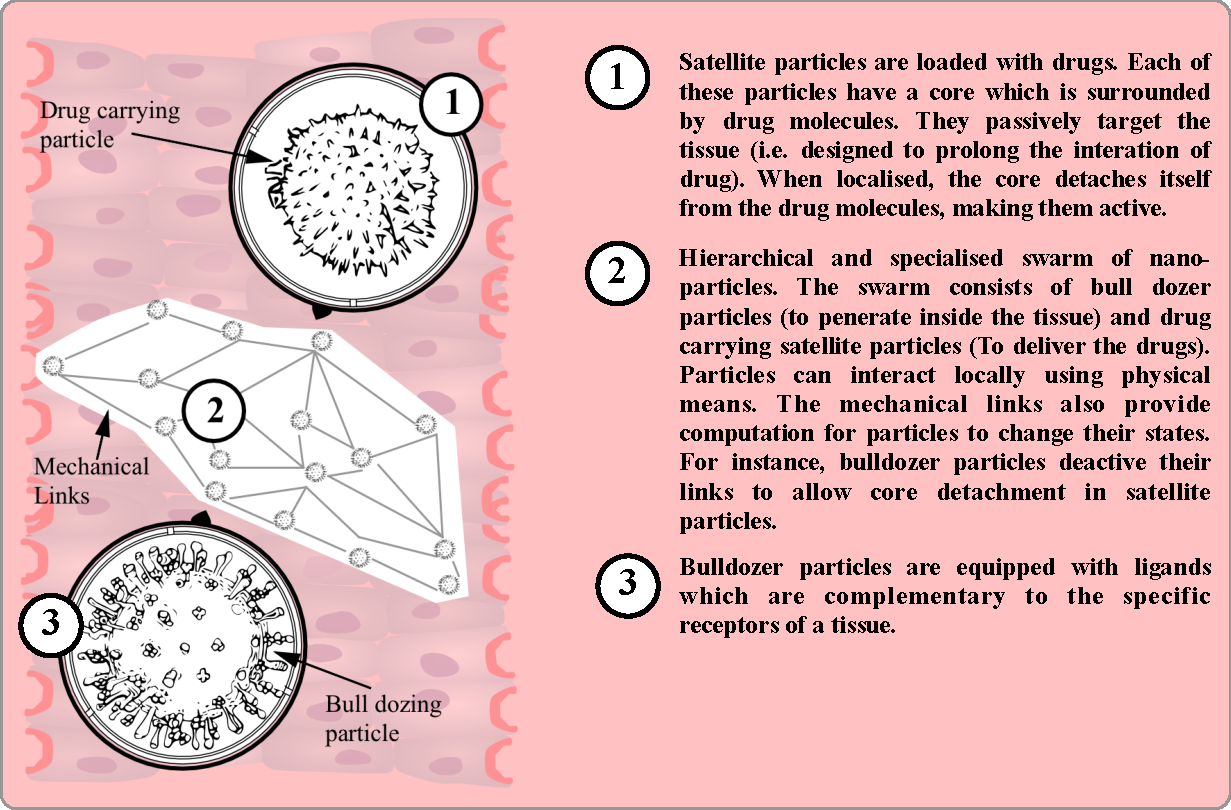
\includegraphics{images/Figure1.pdf}
\caption{A simple hybrid nano-particle systems approach}
\end{figure}

\begin{multicols}{2}
\subsection{A robotic platform for simulating nanoparticle swarms}\label{gen}
Use of robotic swarms to simulate nanoparticle systems, cellular behaviour and targeted drug delivery is a growing trend. The advantage of using real robots rather than simulation is their ability to interact with the real world. In this scenario (nano-medicine), they can also serve the purpose of validating simplified simulation results and complex dynamics of nanoparticles. Furthermore, it is easier to understand the dynamics of such complex systems by realising a hypothesis into physical robots. Moreover, for the case of targeted drug delivery, such robotic platforms must be based on actual biological systems. This type of bio-inspired design is also termed as "wet" nanorobotics\cite{singh2008nanotechnology}. 

Interestingly, there are many animals which follow the principles discussed in earlier section. Siphonophores are the closest related organism to this type of swarm. Like many other colonial hydrozoans in the clade, they asexually reproduce a colony of clonal, physically attached, physiologically specialised bodies (called zooids). Due to a high degree of physiological integration, researchers consider these zooids to be dependent but free-living individuals \cite{mills1995medusae}. Each of these zooids is also functionally specialised (for locomotion, others for feeding, reproducing, digesting, protecting etc.). More interesting is how Siphonophores flawlessly integrate swarm intelligence with the underlying principles of morphological computation, embodiment, and self-organisation. 

Due to their close relation to the desired design objectives, they are the primary inspiration for the design of the proposed robotic platform (Figure 2). Using the robotic platform, logical rules will be abstracted which can then be implemented in the functioning of the aforementioned nanoparticle system (in simulation).
\end{multicols}


\newpage

\begin{figure}[htbp]
\centering
\includegraphics{images/robot design}
\caption{A robotic swarm inspired by Siphonophores.}
\end{figure}
\begin{center}
\section{Literature review}\label{literature}
\end{center}
\begin{multicols}{2}
Use of robotics in the field of nano-medicine and cellular biology to study emergent behaviour is relatively new. However, robotics platforms can serve a great purpose in these studies. For example, in order to test their theory about binding kinetics, Hauert et al., \cite{hauertinsights} divided a kilobot swarm\cite{rubenstein2012kilobot} into two groups (one group represented the target cell and the other; nanoparticles). When initialised, the nanoparticle bots moved randomly until they found and bonded with a cell bot. Although the experiments actually resembled with the behaviour of nanoparticles under the microscope, the swarm (of 1024 individuals) was not actually scaled to the population of nanoparticles (trillions). Thus, a just comparison can't be made to interpret the proposed hypothesis. This issue of scalability is synonymous to the problem of boundary coverage where a swarm of agents is required to deliver some payload to a specific target \cite{williams2006multi}. The problem arises when same level of internal and external noises cause the same agents to behave differently when scaled. For instance, Brownian motion and chemical interactions have been known to affect the swarms differently at nano-scale when the population is increased \cite{jang2004role}.

This also makes it difficult to control the swarms. In a survey paper, Chowdhury et al. \cite{chowdhury2015controlling} categorised control strategies for micro and nano-particles into two groups based on the particle size and the population \footnote{Independent control required no global input (self-organised) and opposite, coupled control exhibited parallel coordination with a global input.}. In both cases, it was observed that chaotic (unpredictable) behaviour emerged even with a population of six particles at nano and micro scales. Furthermore, a huge research gap can be observed (Figure 3) which indicates that there is a need for better control strategies for the particles of nano and micro scales \footnote{Note that Bacteria based approached are not included because they can't be used to realistically simulate the desired emergent behaviour \cite{jain2008nanomedicine}.}. It can also be noted that sensory noise (such as early trigger due to a leaky tumour/target) also affects the robustness. This is especially the case when the nanoparticles passively interact with the tissue. According to a study of medical trial \cite{bae2011targeted}, more than 95 percent of passive nanoparticles end up in spleen, liver, and lungs due to the EPR effect \footnote{Enhanced permeation and retention (EPR) effect refers to the increase in the retention time when the nanoparticles are coated with hydrophilic compunds}. 

An alternative approach can be to instead enforce morphological constraints and utilise the most basic embodiment to overcome noise, scale and size effects. In effect, this approach can also lead to decentralised control. Umedachi et al. developed a soft-bodied robot inspired from the plasmodium of the true slime mold\cite{umedachi2013true}. The true slime mold exhibits an oscillating behaviour (also known as an explore-exploit cycle) which is very similar to CPGs\footnote{Central Pattern generators}. The plasmodium of true slime mold is exchanged throughout the structure for relaying long distance information. Another interesting feature of the true slime mold is that the mass of the plasmodium is conserved \cite{ishiguro2008fully}. Based on these observations, a Real-time tunable spring was developed which mimic the action of plasmodium in an oscillating mold. Furthermore, several RTSs were grouped to share a fixed volume of liquid. To induce the oscillating behaviour, every single unit shared its information with the neighbours using the liquid (every RTS has a force sensor to sense the pressure in the links). Using these complementary features, the robot was able to master the many degrees of freedoms without a centralised control. However, the weighting scheme used to shift the oscillator frequency of individual RTSs required heavy experimentation. A better approach could have been to use neural networks to regulate the resting length of RTSs (CPG inspired ANNs). The salamander-like robot \cite{ijspeert2008central} showcases the level of robustness achieved with a decentralised control based on artificial CPGs (or ANNs). However, designing a CPG for any type of morphology require following inputs. First, the type and number of neuron/oscillators. Second, the type of coupling to take feedback into account. Third, the different types of stimulus. It is relatively easier for deciding these inputs when the number degrees of freedom is small, but it becomes challenging when DOFs increase. Furthermore, there is no fixed method based on which these inputs can be decided for a very large swarm. One way to deal with this is to use reinforcement learning. Furthermore, since the swarms are mechanically constrained, the problem closely resembles to evolving soft robot using powerful generative encoding \cite{Cheney2013UEE24633722463404}.
 
\subsection{Conclusions}\label{literature}
The purpose of this review was to view the trends in targeted drug delivery. It is seen that robotic platforms such as the kilobot are being integrated into the research field. However, there are a few key problems which are needed to be addressed. The issue of scale and size which determine the effectiveness of control mechanisms. It can also be seen that morphological approaches for control strategies have a great potential to overcome these barriers.

\begin{figure}[H]
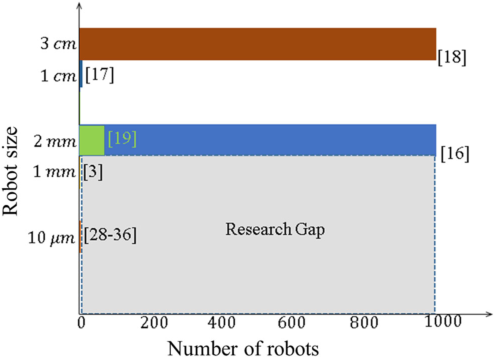
\includegraphics{images/figure_research_gap.pdf}
\caption{Maximum number of robots that can be controlled independently\cite{chowdhury2015controlling}}
\end{figure}
\end{multicols}

\newpage
\section{Risk register}\label{Rregister}
\begin{figure}[htbp]
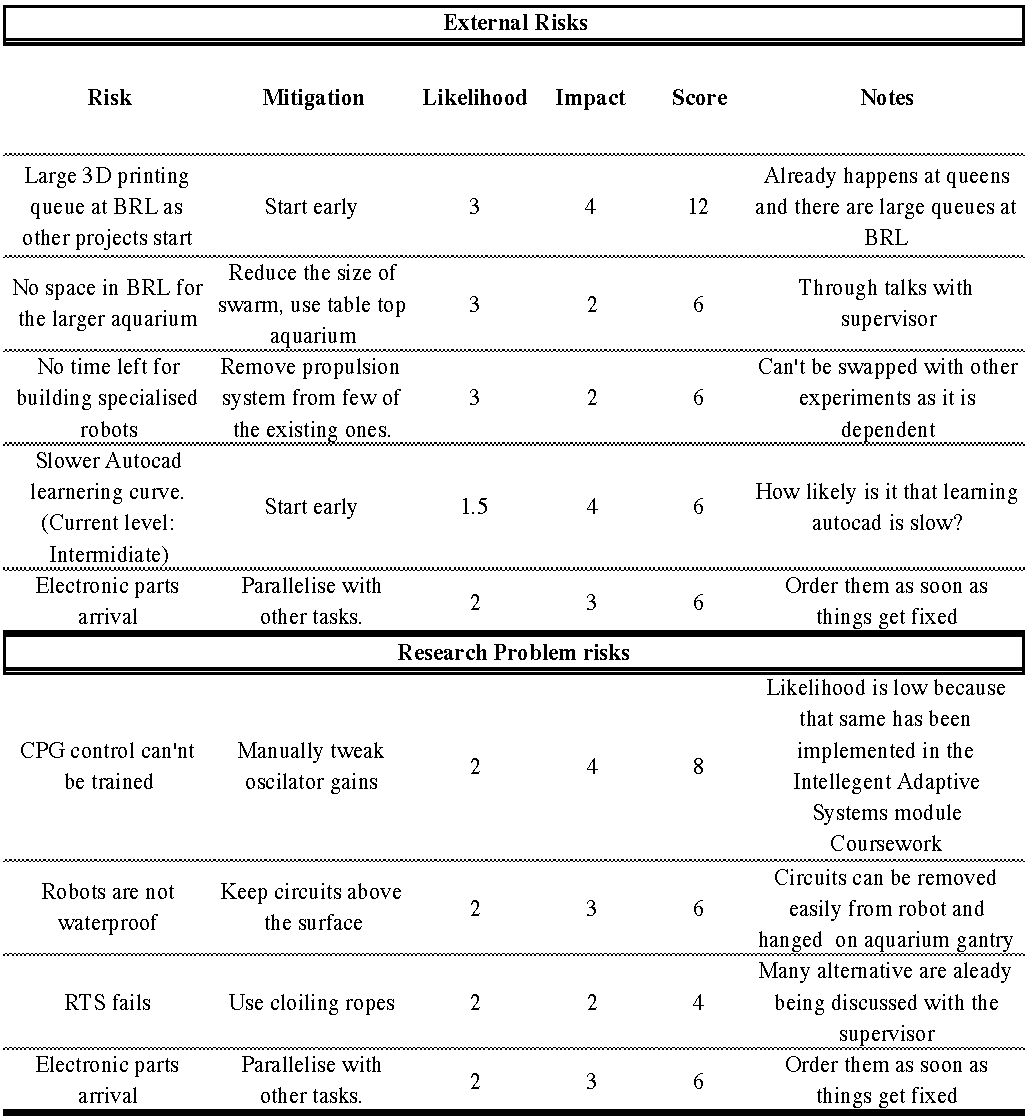
\includegraphics{images/risk.pdf}
\caption{Risk Register}
\end{figure}
\newpage
\section{Timeline}\label{motivation}

\definecolor{barblue}{RGB}{249,100,76}
\definecolor{barbu}{RGB}{76,225, 249}
\definecolor{groupblue}{RGB}{51,102,254}
\renewcommand\sfdefault{phv}
\renewcommand\mddefault{mc}
\renewcommand\bfdefault{bc}
\begin{figure}[htbp]
\centering
\begin{ganttchart}[
  canvas/.append style={fill=none, draw=black!5, line width=.75pt},
  hgrid style/.style={draw=black!5, line width=.75pt},
  vgrid={*1{draw=black!5, line width=.75pt}},
  title/.style={draw=none, fill=none},
  title label font=\bfseries\footnotesize,
  title label node/.append style={below=7pt},
  include title in canvas=false,
  bar label font=\color{black},
  bar label node/.append style={left=0cm},
  bar/.append style={draw=none, fill=barbu},
  bar incomplete/.append style={fill=barblue},
  bar progress label font=\color{black},
  group incomplete/.append style={fill=groupblue},
    group left shift=0,
    group right shift=0,
    group height=.5,
    group peaks tip position=0,
    group label node/.append style={left=0cm}
   ]{1}{24}
  \gantttitle{April}{4}
  \gantttitle{May}{4}
  \gantttitle{June}{4}
  \gantttitle{July}{4}
  \gantttitle{August}{4}
  \gantttitle{September}{4}\\
  \gantttitle[
    title label node/.append style={below left=7pt and -3pt}
  ]{Weeks:\quad1}{1}
  \gantttitlelist{2,...,24}{1} \\
  \ganttgroup[progress=12.5]{Overall}{1}{24} \\
  \ganttbar[
    progress=50,
    name=bar1
  ]{\textbf{\faDesktop}}{1}{3} \\
  \ganttbar[
    progress=30,
    name=bar2
  ]{\textbf{\faConnectdevelop\faCartArrowDown}}{3}{9} \\
  \ganttbar[
    progress=0,
    name=bar4
  ]{\textbf{\faCodepen}}{7}{9} \\
\ganttmilestone[name=m1]{}{8}

\ganttbar[
    progress=0,
    name=bar5,
  ]
{\textbf{\faWrench\faGavel}}{10}{11} \\

\ganttbar[
    progress=0,
    name=bar500,
  ]
{\textbf{\faFlask }}{11}{12} \\


  \ganttbar[
    progress=0,
    name=bar6
  ]{\textbf{\faGear}}{12}{14} \\
  
  \ganttmilestone[name=m2]{}{13}

  \ganttbar[
    progress=0,
    name=bar7
  ]{\textbf{\faGears}}{15}{17} \\

    \ganttmilestone[name=m3]{}{16}

  \ganttbar[
    progress=0,
    name=bar8
  ]{\textbf{\faGe}}{18}{20} \\
  \ganttbar[
    progress=20,
    name=bar9
  ]{\textbf{\faPencil}}{4}{24} \\

  \ganttmilestone{\faBook}{24}{24} \\
  \ganttlink[link mid=.25, link bulge=0.3, link tolerance =0.5]{m1}{bar5}
  \ganttlink[link type=dr]{bar2}{bar5}
  \ganttlink[link type=dr]{bar2}{bar4}
  \ganttlink[link type=dr]{bar5}{bar6}
 \ganttlink[link type=dr]{bar2}{bar6}
 \ganttlink[link type=dr]{bar2}{bar6}
  \ganttlink[link type=dr]{bar6}{bar8}
    \ganttlink[link type=dr]{bar6}{bar7}
  \ganttlink[link type=dr]{bar4}{bar6}
  
\node[fill=white,draw] at ([yshift=-12pt]current bounding box.south){\faDesktop \textnormal{ Simulation, }\faConnectdevelop\faCartArrowDown  \textnormal{ Robot design and parts arrival, }\faCodepen  \textnormal{ Aquarium construction,} \faWrench\faGavel  \textnormal{ Assembly}};

\node[fill=white,draw] at ([yshift=-14pt]current bounding box.south){\faFlask \textnormal{Testing, } \faGear\textnormal{ Objective 2.(a), } \faGears\textnormal{ Objective 2.(b), }\faGe\textnormal{ Objective 2.(c), }\faPencil  \textnormal{ Writeup, }\faBook\textnormal{ Thesis}};


\end{ganttchart}
\caption{Time-line, dependencies and milestones.}
\end{figure}


\newpage
\begin{multicols}{2}
\bibliography{references} 
\bibliographystyle{ieeetr}
\end{multicols}
\end{document}